\documentclass[../../main.tex]{subfiles}

\begin{document}

Wir wissen bereits, dass Aussagen entweder \wahr\  oder \falsch\  sind.
In diesem Abschnitt widmen wir uns der Frage, wie man denn nun herausfinden kann, 
ob eine Aussage \wahr\  oder \falsch\  ist. 

Leider ist das in manchen Fällen gar nicht so einfach oder manchmal sogar 
überhaupt nicht möglich. Das nächste Beispiel zeigt Aussagen, für die es aus verschiedenen Gründen schwierig ist zu entscheiden, ob sie \wahr\  oder \falsch\  sind.

\todo{Besseres Bild für den wütenden Zauberer}
\begin{example}{Aussagen mit schwierig zu bestimmenden Wahrheitswert}
        \parpic[r]{
        
\includegraphics[width=0.1\textwidth]{images/wizard_angry_tmp.png}
    }

    Der Wahrheitswert der Aussage \statement{Der Zauberer ist schlecht gelaunt} hängt davon ab, zu welchem Zeitpunkt diese Aussage getätigt wird. Es gibt nämlich Tage an denen der Zauberer gut gelaunt ist, es gibt aber auch welche an denen er schlecht gelaunt ist.
    \\ \\
    Den Wahrheitswert Aussage \statement{Der Bart vom Zauberer ist nicht echt} könnte man zwar prinzipiell bestimmen, indem man eine Probe seines Barthaares nimmt, jedoch würde der Zauberer dies nicht zulassen (sein Bart ist ihm heilig!).
    \\ \\
    Die Aussage \statement{Der Zaubertrank ist giftig} hat zwar einen Wahrheitswert, jedoch hängt dieser davon ab, auf welchen Zaubertrank sich die Aussage bezieht.
\end{example}

Wir stellen also fest, dass es Aussagen gibt, über die wir nicht ohne weiteres entscheiden können, ob sie \wahr\  oder \falsch\ \  sind. Das Problem ist, dass der Wahrheitswert von manchen Aussagen vom Zeitpunkt der Aufstellung der Aussage abhängt oder der Wahrheitswert vom Kontext abhängt in der die Aussage gestellt wurde. Der Wahrheitswert mancher Aussagen ist zwar im Prinzip bestimmbar, wäre jedoch viel zu aufwendig.

Wir müssen uns also damit abfinden, dass wir im Allgemeinen nicht über den Wahrheitswert einer Aussage entscheiden können. Wir geben uns damit aber noch nicht zufrieden. Können wir zumindest herausfinden, welche Informationen wir mindestens benötigen, um den Wahrheitswert einer Aussage zu bestimmen?

\begin{example}{Atomare Aussagen}
Wir betrachten noch einmal zwei der Aussagen aus dem letzten Beispiel und verknüpfen diese mit \statement{und} zu einer neuen Aussage, die lautet:
\[\statement{Der Zauberer ist schlecht gelaunt und der Zaubertrank ist giftig}\]
Angenommen wir würden die Wahrheitswerte von den beiden kleineren Unteraussagen
\begin{enumerate}
    \item \statement{Der Zauberer ist schlecht gelaunt}
    \item \statement{Der Zaubertrank ist giftig}
\end{enumerate}
kennen, dann könnten wir daraus den Wahrheitswert der gesamten Aussage ableiten. Wüssten wir zum Beispiel, dass der Zauberer schlecht gelaunt ist und, dass der Zaubertrank giftig ist, dann wüssten wir, dass unsere Aussage \statement{Der Zauberer ist schlecht gelaunt und der Zaubertrank ist giftig} \wahr\  ist.
\\ \\
Können wir mit dem gleichen Prinzip auch den Wahrheitswert der beiden Unteraussagen ermitteln? Nein, denn diese beiden Unteraussagen enthalten keine Konnektoren mehr. Sie sind also nicht aus kleineren Aussagen zusammengesetzt. Solche Aussagen, die keine Konnektoren enthalten, nennt man \textbf{atomare Aussagen}.
\end{example}

Tatsächlich sind die einzigen Informationen, die wir benötigen, 
um den Wahrheitswert einer Aussage zu bestimmen, die Wahrheitswerte 
gewisser Unteraussagen. Diese gewissen Unteraussagen sind die sogenannten 
\textbf{atomaren Aussagen}. Das sind Aussagen, die keine Konnektoren enthalten. 
\enquote{Atomar} kommt aus dem griechischen und heißt \enquote{unteilbar}.

\begin{definition} {Atomare Aussage}
Eine \textbf{Atomare Aussage} ist eine Aussage, die keine Konnektoren enthält.
\end{definition}

Im Folgenden lernst du, wie man für beliebige Aussagen den Wahrheitswert 
bestimmen kann, falls man bereits die Wahrheitswerte aller atomaren Aussagen 
dieser Aussage kennt. Wir gehen also davon aus, dass wir zumindest die 
Wahrheitswerte von atomaren Aussagen immer bereits kennen.

Wir können schon mithilfe der Wahrheitswerte von zwei Aussagen $A$ und $B$ 
auch den 
Wahrheitswert von $A \land B$, $A \lor B$, $\lnot A$, $A \implies B$, $A \iff B$
herausfinden, da wir bereits die Bedeutung der Konnektoren kennen. Das wollen
wir uns jetzt genauer anschauen.

\begin{example}{Wahrheitswerte von $\land$}
    Sei $S$ eine Abkürzung für die Aussage \statement{Der Zauberer ist schlecht gelaunt} 
    und $G$ eine Abkürzung für \statement{Der Zaubertrank ist giftig}. Ist der Zauberer 
    tatsächlich schlecht gelaunt ($S$ ist \wahr) und ist der Zaubertrank giftig 
    ($G$ ist auch \wahr), dann ist auch \statement{Der Zauberer ist schlecht gelaunt und
    der Zaubertrank ist giftig}
     (kurz: $S \land G$) \wahr. 
    
    Ist aber entweder $S$ oder $G$ \falsch\  oder sind sogar beide \falsch\ , dann 
    ist $S \land G$ auch \falsch.
    
    Für alle möglichen Fälle der Wahrheitswerte von $S$ und $G$
    können wir nun in einer Tabelle den Wahrheitswert von $S \land G$ angeben.
    
    \[\begin{array}{cc s c}\toprule
        S & G & S \land G\\\midrule
        \falsch   & \falsch   & \falsch  \\
        \falsch   & \wahr & \falsch\\
        \wahr & \falsch   & \falsch\\
        \wahr & \wahr & \wahr\\\bottomrule
    \end{array}\]
\end{example}

\textbf{Wahrheitswerte von dem Konnektor $\land$}:
Seien $A,B$ zwei beliebige Aussagen (z.B. die aus letztem Beispiel). Angenommen, wir kennen die 
Wahrheitswerte von $A$ und $B$, dann können wir daraus
den Wahrheitswert für $A \land B$ folgern.  $A \land B$ ist nämlich genau dann \wahr, wenn sowohl $A$ als auch 
$B$ \wahr\  ist. Ist also $A$ oder $B$ \falsch\  oder sind sogar beide \falsch\ ,
dann ist auch $A \land B$ \falsch\ .

Auf die gleiche Weise können wir auch bei Aussagen in denen die anderen Konnektoren
aus dem letzten Abschnitt vorkommen, herausfinden, wann sie \wahr\ sind. Dies schauen wir
uns als nächstes für den Konnektor $\lor$ an.
\begin{example}{Wahrheitswerte von $\lor$}
    Sei $S$ wieder die Abkürzung für die Aussage \statement{Der Zauberer ist schlecht 
    gelaunt} und $G$ wieder die Abkürzung für \statement{Der Zaubertrank ist giftig}. 
    Ist mindestens eine Aussage der Aussagen $S, G$  \wahr, dann ist auch 
    \statement{Der Zauberer ist schlecht gelaunt und der Zaubertrank ist giftig}
    (kurz: $S \lor G$) \wahr. 
    
    Ist also zum Beispiel der Zauberer nicht schlecht gelaunt ($S$ ist \falsch\ ), aber 
    der Zaubertrank ist giftig ($G$ ist \wahr), dann ist $S \lor G$ \wahr. 
    
    $S \lor G$ kann nur \falsch\  werden, wenn der Zauberer nicht schlecht gelaunt 
    ist ($S$ ist \falsch) und der Zaubertrank nicht giftig ist ($G$ ist \falsch). 
    
    Für 
    alle möglichen Fälle der Wahrheitswerte von $S$ und $G$
    können wir nun in einer Tabelle den Wahrheitswert von $S \lor G$ angeben.
    
    \[\begin{array}{cc s c}\toprule
        S & G & S \lor G\\\midrule
        \falsch   & \falsch   & \falsch  \\
        \falsch   & \wahr & \wahr\\
        \wahr & \falsch   & \wahr\\
        \wahr & \wahr & \wahr\\\bottomrule
    \end{array}\]
\end{example}

\textbf{Wahrheitswerte von dem Konnektor $\lor$}: Seien nun $A,B$ zwei beliebige 
Aussagen (z.B. die aus letztem Beispiel)). 
Angenommen wir kennen die Wahrheitswerte von $A$ und $B$, 
dann können wir den Wahrheitswert von $A \lor B$ folgern. $A \lor B$ ist nämlich 
genau dann \wahr, wenn 
mindestens eine der Aussagen $A,B$ \wahr\  ist. Insbesondere ist $A \lor B$ auch 
\wahr\  wenn $A$ und $B$ beide gleichzeitig \wahr\  sind. Der einzige Fall in dem 
 $A \lor B$ \falsch\  wird, ist, wenn sowohl $A$ als auch $B$ beide \falsch\  sind.

 Wir stellen nun diesselben Überlegungen zu den Wahrheitswerten nun für den Konnektor
 $\lnot$ an.
\begin{example}{Wahrheitswerte von $\lnot$}
Sei $G$ noch einmal die Abkürzung für die Aussage \statement{Der Zaubertrank ist giftig}. 
Ist der Zaubertrank wirklich giftig ($G$ ist \wahr), dann ist die Negation \statement{Der Zaubertrank ist nicht giftig} (kurz: $\lnot G$) \falsch. Ist aber 
andersherum $G$ \falsch, dann ist $\lnot G$ \wahr. 

Für die zwei Fälle der Wahrheitswerte von $G$
können wir nun in einer Tabelle den Wahrheitswert von $\lnot G$ angeben.
    \[\begin{array}{c s c}\toprule
        G & \lnot G\\\midrule
        \falsch & \wahr\\
        \wahr & \falsch\\\bottomrule
    \end{array}\]
\end{example}

\textbf{Wahrheitswerte von $\lnot$}: Zur Erinnerung: Verneinen wir eine Aussage, 
dann ist das die Negation der ursprünglichen Aussage. Ist $A$ eine beliebige  
Aussage (z.B. die aus letztem Beispiel), dann notieren wir die Negation von $A$ durch $\lnot A$. Eine Negation 
dreht den Wahrheitswert der Aussage um. Das heißt, wenn die Aussage \wahr\  ist, 
dann ist ihre Negation \falsch\  und ist eine Aussage \falsch\ , dann ist 
ihre Negation \wahr.

Wir wiederholen die gleichen Überlegungen nun für den Konnektor $\iff$.
\begin{example}{Wahrheitswerte von $\iff$}
    Sei $F$ eine Abkürzung für die Aussage 
    \statement{Der Zaubertrank verleiht Superkräfte} und $S$ wieder die Abkürzung 
    für \statement{Der Zauberer ist schlecht gelaunt}. Verleiht zum Beispiel der 
    Zaubertrank keine Superkräfte (also $F$ ist \falsch) und ist der Zauberer nicht 
    gut gelaunt ($G$ ist \falsch), dann ist trotzdem \statement{Der Zaubertrank verleiht Superkräfte
    genau dann wenn der Zauberer schlecht gelaunt ist}(kurz: $F \iff G$) \wahr, da $F$ und $G$ 
    den gleichen Wahrheitswert besitzen. 
    
    Verleiht der Zaubertrank Superkräfte ($F$ ist \wahr) und ist der Zauberer 
    schlecht gelaunt ($G$ ist \falsch), dann ist $F \iff G$ \falsch, da die 
    Wahrheitswerte von $F$ und $G$ unterschiedlich sind. 
    
    Für alle möglichen Fälle der 
    Wahrheitswerte von $F$ und $G$
    können wir nun in einer Tabelle den Wahrheitswert von $F \iff G$ angeben.
    
    \[\begin{array}{cc s c}\toprule
        F & G & F \iff G\\\midrule
        \falsch   & \falsch   & \wahr  \\
        \falsch   & \wahr & \falsch\\
        \wahr & \falsch   & \falsch\\
        \wahr & \wahr & \wahr\\\bottomrule
    \end{array}\]
\end{example}

\textbf{Wahrheitswerte von dem Konnektor $\iff$}: Seien nun $A,B$ zwei beliebige 
Aussagen (z.B. die aus letztem Beispiel) von denen wir den
Wahrheitswert kennen. Wir können den Wahrheitswert von
 $A \iff B$ folgern. $A \iff B$ ist nämlich genau dann \wahr\  ist, wenn $A$ denselben Wahrheitswert 
 wie $B$ besitzt. 

 Zum Schluss müssen wir dieselben Überlegungen wie bisher noch für den Konnektor
 $\implies$ anstellen.
\begin{example}{Wahrheitswerte von $\implies$}
    Sei $G$ wieder die Abkürzung für die Aussage \statement{Der Zauberer ist schlecht 
    gelaunt} und $F$ wieder die Abkürzung für \statement{Der Zaubertrank verleiht 
    Superkräfte}. 
    Ist beispielsweise der Zauberer nicht gut gelaunt ($G$ ist \falsch) und der 
    Zaubertrank verleiht auch keine Superkräfte ($F$ ist \falsch), dann ist 
    \statement{Wenn der Zauberer schlecht gelaunt ist, dann verleiht der Zaubertrank Superkräfte}
    (kurz: $G \implies F$) \wahr.
    
    $G\implies F$ wird nur \falsch, wenn der Zauberer gut gelaunt 
    ist ($G$ ist \wahr) aber trotzdem der Trank keine Superkräfte verleiht 
    ($F$ ist \falsch).
    
    Für alle möglichen Fälle der Wahrheitswerte von $G$ und $F$
    können wir nun in einer Tabelle den Wahrheitswert von $G \implies F$ angeben.
    
    \[\begin{array}{cc s c}\toprule
        G & F & G \implies F\\\midrule
        \falsch   & \falsch   & \wahr  \\
        \falsch   & \wahr & \wahr\\
        \wahr & \falsch   & \falsch\\
        \wahr & \wahr & \wahr\\\bottomrule
    \end{array}\]
\end{example}

\textbf{Wahrheitswerte von dem Konnektor $\implies$}: 
Seien $A,B$ wieder zwei beliebige  Aussagen (z.B. die aus dem letztem Beispiel)
. Kennen wir die Wahrheitswerte von $A$ und $B$, dann können
wir daraus den Wahrheitswert von $A \implies B$ folgern. 
Dazu interpretiert man die Aussage $A \implies B$ 
als ein Versprechen. Nur wenn dieses Versprechen explizit gebrochen wird, wird
$A \implies B$ \falsch. Das Versprechen ist nun, dass wenn $A$ \wahr\  
ist, dann muss auch $B$ \wahr. Wenn $A$ \falsch\  ist, dann ist dem Versprechen 
egal, was mit $B$ passiert. Das Versprechen wird also nur gebrochen, wenn $A$ 
\wahr\  ist, aber $B$ \falsch\  ist.

Wir haben jetzt Konnektor für Konnektor herausgefunden, welche Wahrheitswerte wir
erhalten wenn wir Aussagen mit ihnen verknüpfen. 
Wir haben dabei die Konnektoren $\land,\lor,\implies,\iff,\lnot$ untersucht. 
Die folgende Tabelle fasst nochmal alle vorangegangen Wahrheitswerte in einer Tabelle 
zusammen.
\begin{definition}{Wahrheitswerte aller Konnektoren}
\label{whw}
Seien $A,B$ zwei beliebige Aussagen. Der Wahrheitswert aller möglichen Verknüpfungen dieser beiden Aussagen ist dann wie folgt definiert.

    \[\begin{array}{cc s ccccc}\toprule
        A & B & A \land B & A\lor B & A\implies B & A\iff B & \lnot A\\\midrule
        \falsch & \falsch & \falsch & \falsch & \wahr & \wahr & \multirow{2}{*}{\wahr}\\
        \falsch & \wahr & \falsch & \wahr & \wahr & \falsch &  \\
         \wahr & \falsch & \falsch & \wahr & \falsch & \falsch & \multirow{2}{*}{\falsch}
        \\
        \wahr & \wahr & \wahr & \wahr & \wahr & \wahr & 
         \\\bottomrule
    \end{array}\]
\end{definition}

Zu Beginn dieses Kapitels wurde erwähnt, dass die Wahrheitswerte von atomaren 
Unteraussagen einer völlig beliebigen Aussage die einzigen Informationen sind, die wir 
benötigen, um den Wahrheitswert der Aussage zu ermitteln. Wie man das macht, lernst
du jetzt kennen.

Tatsächlich ist die Vorgehensweise, die wir gleich zeigen, nichts neues und funktioniert 
ähnlich zu einem Verfahren, das man bereits im Schlaf beherrscht: 
Dem Auswerten von Termen. Das nächste Beispiel wiederholt dies und dröselt die Schritte, die man dabei vornimmt, auf.

\todo{abbildung tikzen}
\begin{example}{Termauswertung}
Stell dir vor, deine Aufgabe ist es, den Term $x \cdot (y - (z \cdot z))$ auszuwerten
 und du weißt, dass $x = 3$, $y = 7$ und  $z = 2$ ist.
Um den Wert von $x \cdot (y - (z \cdot z))$ heraufzufinden, gehst
du wie folgt vor:
\begin{enumerate}
    \item Du ersetzt die Variablen im Term durch ihre Werte:
    \[x \cdot (y - (z \cdot z)) \longmapsto 3 \cdot (7 - (2 \cdot 2)) \]
    
    \item Anschließend ersetzt du solange einen Teilterm, den du direkt ausrechnen 
    kannst, durch sein Ergebnis, bis nur noch das Gesamtergebnis übrig bleibt.
    
    
    Die nächste Abbildung zeigt genau dieses Vorgehen. Dabei ist in jeder Zeile blau markiert welcher Teilterm gewählt und dann ersetzt wurde.
    \begin{center}
        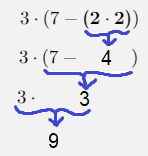
\includegraphics[width=0.275\textwidth]{images/TEMP_termalg.png}
    \end{center}
\end{enumerate}
    Es bleibt am Ende nur noch 9 übrig. Wir haben damit herausgefunden, 
    dass für unsere eingesetzten Werte $x \cdot (y - (z \cdot z)) = 9$ ist.

\end{example}

Und genau diese Vorgehensweise, die wir beim Auswerten von Termen benutzen, 
lässt sich auf gleiche Art und Weise auf das Auswerten von Aussagen übertragen. 
Es kommen nämlich genau dieselben Schritte vor. Möchte man nämlich den Wahrheitswert einer Aussage bestimmen, dann führt man folgende zwei Schritte aus:
    \begin{enumerate}
    \item Ersetze alle atomaren Aussagen durch ihren Wahrheitswert.
    \item Werte Paare oder einzelne Wahrheitswerte, die direkt mit einem Konnektor
        verknüpft sind aus, bis nur noch ein Wahrheiswert übrig bleibt.
    \end{enumerate}
    
\todo{die abbildung tikzen}
\begin{example}{Wahrheitswertbestimmung}
Seien $A, B, C$ drei atomare Aussagen. Wenn wir wissen, dass $A$ \wahr\  ist, $B$ \wahr\  ist und $C$ \falsch\   ist, was ist dann der Wahrheitswert folgender Aussage?
\[A \land ( (\lnot B) \lor C)\]
Wir wenden das eben beschriebene Verfahren an.
\begin{enumerate}
    \item Zunächst ersetzen wir alle atomaren Aussagen durch ihren Wahrheitswert:
    \[A \land ( (\lnot B) \lor C) \longmapsto  \wahr \land ((\lnot \wahr) \lor \falsch)\]
    \item Jetzt werten wir Paare oder einzelne Wahrheitswerte, 
    die direkt mit einem Konnektor verknüpft sind aus, bis nur noch ein einzelner Wahrheitswert
    übrig bleibt.
    
    Die nächste Abbildung zeigt wie dieses Vorgehen für die 
    Aussage 
    
    $A \land ( (\lnot B) \lor C)$ aussieht:

\begin{center}
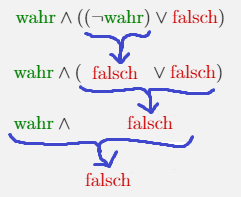
\includegraphics[width=0.4\textwidth]{images/TEMP_wahrheitsalg.png}
\end{center}

In jeder Zeile ist 
    dabei blau gekennzeichnet, welcher Wahrheitswert bzw. welches Paar von 
    Wahrheitswerten gewählt und dann ersetzt wurde. 
\end{enumerate}
Es bleibt nur noch \falsch\  übrig. Unsere Aussage $A \land ( (\lnot B) \lor C)$ ist also
\falsch, wenn $A$ und $B$ \wahr\ sind und $C$ \falsch\ ist.
\end{example}
Wenn wir von einer Aussage $A$ die Wahrheitswerte ihrer atomaren Unteraussagen
kennen, wissen wir jetzt also, wie wir den Wahrheitswert von $A$ ermitteln können. 
Kennt man die Wahrheitswerte der atomaren Unteraussagen aber nicht, kann man $A$ 
trotzdem analysieren, indem man für alle Kombinationen der möglichen Wahrheitswerte 
der atomaren Unteraussagen den Wahrheitswert von $A$ angibt.

\begin{example}{Wahrheitstabelle}
Wir analysieren die Aussage 
$A \land ( (\lnot B) \lor C)$
aus letztem Beispiel.
Die Aussage enthält die atomaren Aussagen $A,B,C$. Wir listen jetzt
tabellarisch den Wahrheitswert der Aussage für alle möglichen Kombinationen der 
Wahrheitswerte von $A$,$B$ und $C$ auf.

In der Tabelle sind als Hilfestellung noch die Wahrheitswerte aller 
Unteraussagen für jede Variablenbelegung angegeben. Das wäre aber nicht nötig 
gewesen. Die 7. Zeile entspricht den Wahrheiswerten, die wir im letzten Beispiel 
verwendet haben. 
    \[\begin{array}{ccc s ccc}\toprule
        A & B & C & \lnot B & (\lnot B) \lor C&A \land (\lnot B \lor C)\\\midrule
        \falsch & \falsch & \falsch &  \wahr& \wahr&\falsch \\
        \falsch & \falsch & \wahr &  \wahr& \wahr &\falsch \\
        \falsch & \wahr & \falsch & \falsch& \falsch &\falsch \\
        \falsch & \wahr & \wahr &\falsch & \wahr &\falsch \\
        \wahr & \falsch & \falsch &  \wahr& \wahr &\wahr \\
        \wahr & \falsch & \wahr & \wahr & \wahr &\wahr \\
        \wahr & \wahr & \falsch & \falsch& \falsch&\falsch \\
        \wahr & \wahr & \wahr & \falsch& \wahr &\wahr \\
        \bottomrule
    \end{array}\]
Solch eine Tabelle nennt sich eine \textbf{Wahrheitstabelle} für die Aussage $A \land ( (\lnot B) \lor C)$.

\end{example}
Listen wir alle Kombinationen der Wahrheitswerte der atomaren Aussagen von $A$, zusammen mit den entsprechenden Wahrheitswerten von $A$ tabellarisch auf, dann nennen wir dies eine \textbf{Wahrheitstabelle} für $A$. 

\begin{definition}{Wahrheitstabelle}
Ist $A$ eine Aussage und kommen in $A$ die atomaren Unteraussagen $x_1,\dots,x_n$ vor, dann nennen wir eine Tabelle, die für alle möglichen Kombinationen der Wahrheitswerte von $x_1,\dots,x_n$ den Wahrheitswert von $A$ angibt, eine \textbf{Wahrheitstabelle} für $A$.
\end{definition}

Prinzipiell kann man für jede Aussage eine Wahrheitstabelle aufstellen. 
In der Praxis gibt es aber Aussagen, für die das aber nicht unbedingt 
sinnvoll ist, da die Wahrheitswerte der atomaren Aussagen offensichtlich sind 
und es sich daher nicht lohnt, Fälle durchzuspielen, in denen die atomaren 
Aussagen andere Wahrheitswerte annehmen. Das könnte ja sowieso nicht eintreten. 
Ein Beispiel hierfür ist die Aussage: \statement{1 ist gleich 1 oder 1 ist gleich 1}. 
Den Fall durch zuspielen, dass \statement{1 ist gleich 1}, \falsch\ ist, wäre zwar 
prinzipiell möglich, ist aber wenig sinnvoll, denn wir wissen ja, dass die Aussage \wahr\  ist.

Wir wollen jetzt unser neu gewonnenes Wissen nutzen, um das Logikrätsel aus 
der Einleitung systematisch zu lösen.

\begin{example}{Lösung Logikrätsel}
    \parpic[r]{
        
\includegraphics[width=0.2\textwidth]{images/wizard.png}
    }
    
    Wiederholung des Rätsels: \textit{Ein Zauberer gibt dir einen Zaubertrank, 
    der entweder giftig ist oder dir Flügel verleiht. Der Zauberer sagt entweder 
    immer die Wahrheit oder lügt immer.}
    
    \textit{Er gestattet dir \emph{eine} Frage, um herauszufinden, ob der 
    Zaubertrank giftig ist oder dir Flügel verleiht.}
    
    \picskip{1}
     \textbf{Welche Frage musst du dem Zauberer also stellen, um herauszufinden, ob der Trank giftig ist?}
    
    Lösung des Rätsels: Wir können die Gesamtsituation auch so auffassen, dass 
    wir dem Zauberer
    eine Aussage nennen. Wenn der Zauberer die Wahrheit sagt, dann nennt er uns den 
    echten
    Wahrheitswert der Aussage
    und wenn der Zauberer lügt, dann nennt er uns den falschen. Wir tragen einmal in einer Tabelle die verschiedenen
     Fälle zusammen, die auftreten können. $A$ steht dabei für den echten Wahrheitswert
     unser Aussage (die wir jetzt noch nicht kennen), $L$ dafür, ob der Zauberer
     lügt und $Z$ für den Wahrheitswert, den uns der Zauberer nennt. 
    
     \[\begin{array}{cc s c}\toprule
        A & L & Z\\\midrule
        \falsch & \falsch &\falsch  \\
        \falsch & \wahr &\wahr  \\
        \wahr & \falsch &\wahr  \\
        \wahr & \wahr &\falsch  \\
        \bottomrule
    \end{array}\]

    Wir wollen unsere Aussage so wählen, dass wir mit dem Wahrheitswert, den uns 
    der Zauberer
    nennt, herausfinden können, ob der Trank giftig ist. Konkret: Ist der Trank
    giftig, dann wollen wir dass der Wahrheitswert vom Zauberer \wahr\  ist und wenn der Trank
    Flügel verleiht (also nicht giftig ist), dann soll der Wahrheitswert vom Zauberer \falsch\  sein, unabhängig
    davon ob der Zauberer lügt oder nicht. Wir halten diese Forderung in einer Tabelle fest.
    $G$ steht für \statement{Giftig} und $L$, $Z$ wie oben.

    \[\begin{array}{cc s c}\toprule
        G & L & Z\\\midrule
        \falsch & \falsch & \falsch  \\
        \falsch & \wahr & \falsch  \\
        \wahr & \falsch & \wahr  \\
        \wahr & \wahr & \wahr  \\
        \bottomrule
    \end{array}\]

    Daraus können wir bereits schließen, welche Wahrheitswerte die Aussage, die wir dem Zauberer 
    nennen, in Abhängigkeit von $G$ und $L$ haben muss. 
    Wir müssen dazu nämlich nur die Wahrheitswerte in den Fällen umdrehen, in denen der 
    Zauberer lügt. Im Fall $G$ \falsch\ und $L$ \wahr\  wollen wir zum Beispiel, dass
    die Antwort vom Zauberer \falsch\ ist. Da der Zauberer aber lügt, muss unsere
    Aussage in diesem Fall also \wahr\ sein.
    
    Wir ergänzen die letzte Tabelle jetzt also um die Spalte $A$, die
    die Wahrheitswerte enthält, die unsere Aussage haben muss. Die markierten Wahrheitswerte
    in der Spalte von $A$ sind genau die, in denen wir den Wahrheitswert von $G$ negiert haben,
    weil in dem Fall der Zauberer lügt.

    \[\begin{array}{cc s cc}\toprule
        G & L & A &Z\\\midrule
        \falsch & \falsch & \falsch &\falsch  \\
        \falsch & \wahr & \underline{\textbf{\wahr}} &\falsch  \\
        \wahr & \falsch & \wahr &\wahr  \\
        \wahr & \wahr & \underline{\textbf{\falsch}} &\wahr  \\
        \bottomrule
    \end{array}\]

    Denkt man sich die Spalte $Z$ weg, dann ist die letzte Tabelle eine Wahrheitstabelle
    für die Aussage, die wir dem Zauberer nennen wollen. Wir müssen jetzt also nur
    noch eine Aussage finden, die zu dieser Wahrheitstabelle passt.
    Das schaffen wir, indem wir uns anschauen, in welchen Fällen die Aussage \wahr\  sein soll.
    Die Aussage, die wir suchen, sagt dann aus, ob mindestens einer dieser Fälle eintritt.
    Konkret: Die Fälle, in denen die Aussage \wahr\  werden soll sind:
    \begin{enumerate}
        \item $G$ \falsch\ , $L$ \wahr\
        \item $G$ \wahr\ , $L$ \falsch
    \end{enumerate}
    Dass der 1. Fall eintritt, formulieren wir durch
    $\lnot G \land L$ und dass der 2. Fall eintritt durch $G \land \lnot L$. 
    Und dass mindestens einer dieser Fälle eintritt, lässt sich durch
    \[ (\lnot G \land L) \lor (G \land \lnot L)\]
    beschreiben.
    Das ist genau die Aussage, die wir gesucht haben und damit auch die Lösung unseres
    Rätsels. Natürlichsprachlich formuliert würden wir den Zauberer also fragen:

    \textbf{(Ist der Trank nicht giftig und lügst du) oder (ist der Trank giftig und lügst du nicht) ?}
    
    Egal ob der Zauberer nun lügt oder nicht, wir haben diese Frage bzw. Aussage so konstruiert,
    dass der Zauberer mit \textit{Nein} bzw. \falsch\ antworten wird, wenn 
    der Trank nicht giftig ist
    und mit \textit{Ja} bzw. \wahr\ antworten wird, wenn der Trank
    giftig ist.

\end{example}

\begin{nutshell}{Wahrheitstabellen}
    Eine \textbf{atomare Aussage} ist eine Aussage, die keine Konnektoren enthält. \bigskip
   
    Eine \textbf{Wahrheitstabelle} einer Aussage gibt für alle möglichen Kombinationen der Wahrheitswerte der atomaren Unteraussagen an, was der Wahrheitswert der Aussage ist.\bigskip

    Seien $A,B$ beliebige Aussagen. Die folgende Tabelle definiert für alle Konnektoren den Wahrheitswert der Verknüpfung von $A,B$.
    \[\begin{array}{cc s ccccc}\toprule
        A & B & A \land B & A\lor B & A\implies B & A\iff B & \lnot A\\\midrule
        \falsch & \falsch & \falsch & \falsch & \wahr & \wahr & \multirow{2}{*}{\wahr}\\
        \falsch & \wahr & \falsch & \wahr & \wahr & \falsch &  \\
         \wahr & \falsch & \falsch & \wahr & \falsch & \falsch & \multirow{2}{*}{\falsch}
        \\
        \wahr & \wahr & \wahr & \wahr & \wahr & \wahr & 
         \\\bottomrule
    \end{array}\]
    \\ \\
    Möchte man den Wahrheitswert einer Aussage bestimmen und kennt man die Wahrheitswerte ihrer atomaren Aussagen, dann geht man wie folgt vor:
    \begin{enumerate}
    \item Ersetze alle atomaren Aussagen durch ihren Wahrheitswert.
    \item 
    Werte Paare oder einzelne Wahrheitswerte, die direkt mit einem Konnektor
    verknüpft sind aus, bis nur noch ein Wahrheiswert übrig bleibt.
    \end{enumerate}

\end{nutshell}

\end{document}
